\section{Commonsense for Zero-Shot NLVL}
\label{sec:proposedSection}

\subsection{Problem Formulation}
We denote an input video as $V$, and its grounding annotations as \(\left( Q,V_{\text{span}}\right) \), where $Q$ is the query representation and \(V_{\text{span}}\!=\!\left( t_{s},t_{e}\right)\) is the corresponding video moment span annotation, with \(t_{s}\) and \(t_{e}\) representing the start and end timestamps, respectively. Learning to localize a video moment conditioned on a query entails maximizing the expected log-likelihood of the model parameterized by \(\theta\). In its typical setting, this can be formulated as follows:
\begin{equation}
\label{eq:groundingOriginal}
    \theta ^{\ast }=\arg \max _{\theta } \mathbb{E}\left[ \log p_{\theta }\left(  V_{\text{span}} | V,Q\right) \right]. 
\end{equation}
In the zero-shot setting, the goal is to learn this task without parallel video-query annotations. Hence, the query and video moment annotations are derived from $V$, using a dynamic video moment proposal method followed by a pseudo-query generation mechanism. Formally,  \(V_{\text{span}}\,\!{=}\!\,f_{\text{span}}(V)\) and \(Q\,\!{=}\!\,f_{pq}(V_{\text{span}})\), where $f_{\text{span}}$ and $f_{\text{pq}}$ are video moment proposal and pseudo-query generation mechanisms, respectively. Given that $f_{\text{span}}$ and $f_{\text{pq}}$ are responsible for generating the annotations, the performance of the localization model heavily depends on the quality of these modules. Existing methods face challenges in aligning \(Q\) to \(V_{\text{span}}\) due to noise introduced by ungrounded pseudo-query generation mechanisms. 
To address this, we simplify \(f_{\text{pq}}\) while augmenting cross-modal understanding by leveraging external information in the form of a commonsense graph \(G_{C}(C, E)\) with \(n_c\) nodes, where \(C\!=\!\left\{c_{1}, c_{2}, \dots, c_{n_{C}}\right\}\) are the concept node vector representations and \(E\) is the set of weighted directed edges, respectively. Accordingly, learning can be formulated as
\begin{equation}
\label{eq:groundingOurs}
    \theta ^{\ast }=\arg \max _{\theta } \mathbb{E}\left[ \log p_{\theta }\left(  V_{\text{span}}| V,Q,G_{C}\right) \right].
\end{equation}

\noindent Figure \ref{fig:approach} shows both training and inference flows.
\subsection{Pseudo-supervised Setup}
\modelname first processes a raw video with a video moment proposal $f_{\text{span}}$ module that extracts important video segments capturing key events, and a pseudo-query generation $f_{\text{pq}}$ that generates text query annotations corresponding to the extracted video segments.

\paragraph{Dynamic Video Moment Proposal ($f_{\text{span}}$).}
We adopt the dynamic video moment proposal approach proposed by \citet{nam_zero-shot_2021}. Specifically, $f_{\text{span}}$ primarily comprises a k-means clustering mechanism that groups semantically similar and temporally proximal video frame features together to extract atomic moments. To obtain frame features, we consider the columns of a frame-wise similarity matrix derived from the CNN features of individual frames. We enforce temporal proximity by concatenating the frame index to the features. Composite video moments are then formed by combining neighboring atomic moments, and a subset of all possible combinations is sampled uniformly at random. The resulting set of video moments corresponds to $V_{\text{span}}$.

\paragraph{Pseudo-query Generation ($f_{\text{pq}}$).} The pseudo-query is constructed as a collection of objects present in the video. To generate the pseudo-query, we employ an off-the-shelf object detector, enabling the extraction of pertinent objects in \(V_{\text{span}}\). We adopt a top-$k$ strategy to sample the $k$ most probable object predictions associated with the query \query.

\paragraph{Video Encoder.}
We uniformly sample $T$ frames from $V$ and extract their CNN (\eg, I3D~\cite{qian_locate_2022}) features. These features are contextually encoded using a video encoder ${\phi}_{v}$ to yield frame features ${\phi}_{v}(V)\!=\!\left\{ v_{1},v_{2},\ldots,v_{T}\right\}$ where $v_{i}\in\mathbb{R}^{d}$, and $d$ is the common video/query encoding dimension. We implement ${\phi}_{v}$ as a GRU-based encoder.

\paragraph{Query Encoder.}
Our pseudo-query $Q$, composed of up to $k$ tokens, is encoded using a query encoder ${\phi}_{q}$ that generates query embeddings ${\phi}_{q}(Q)\!=\!\left\{ q_{1},q_{2},\ldots,q_{k}\right\}$, for the top-$k$ detected objects extracted from the pseudo-query generation. Here, $q_{i}\in \mathbb{R}^{d}$ and $d$ is the common video/query encoding dimension. We implement ${\phi}_{q}$ as a bi-directional GRU-based encoder preceded by a trainable embedding layer. 

\subsection{Commonsense Enhancement Module}
\label{sec:cem}
To enrich the encoded video and query features with information grounded in commonsensical knowledge, we introduce a Commonsense Enhancement Module (CEM), pictorially described in Figure~\ref{fig:cem}. This enhancement helps inject necessary information into video and query representations, which can not just help bridge the gap between the available visual and textual cues but also provide rich information to the downstream span localization module. 

\begin{figure}[t!]
    \centering
    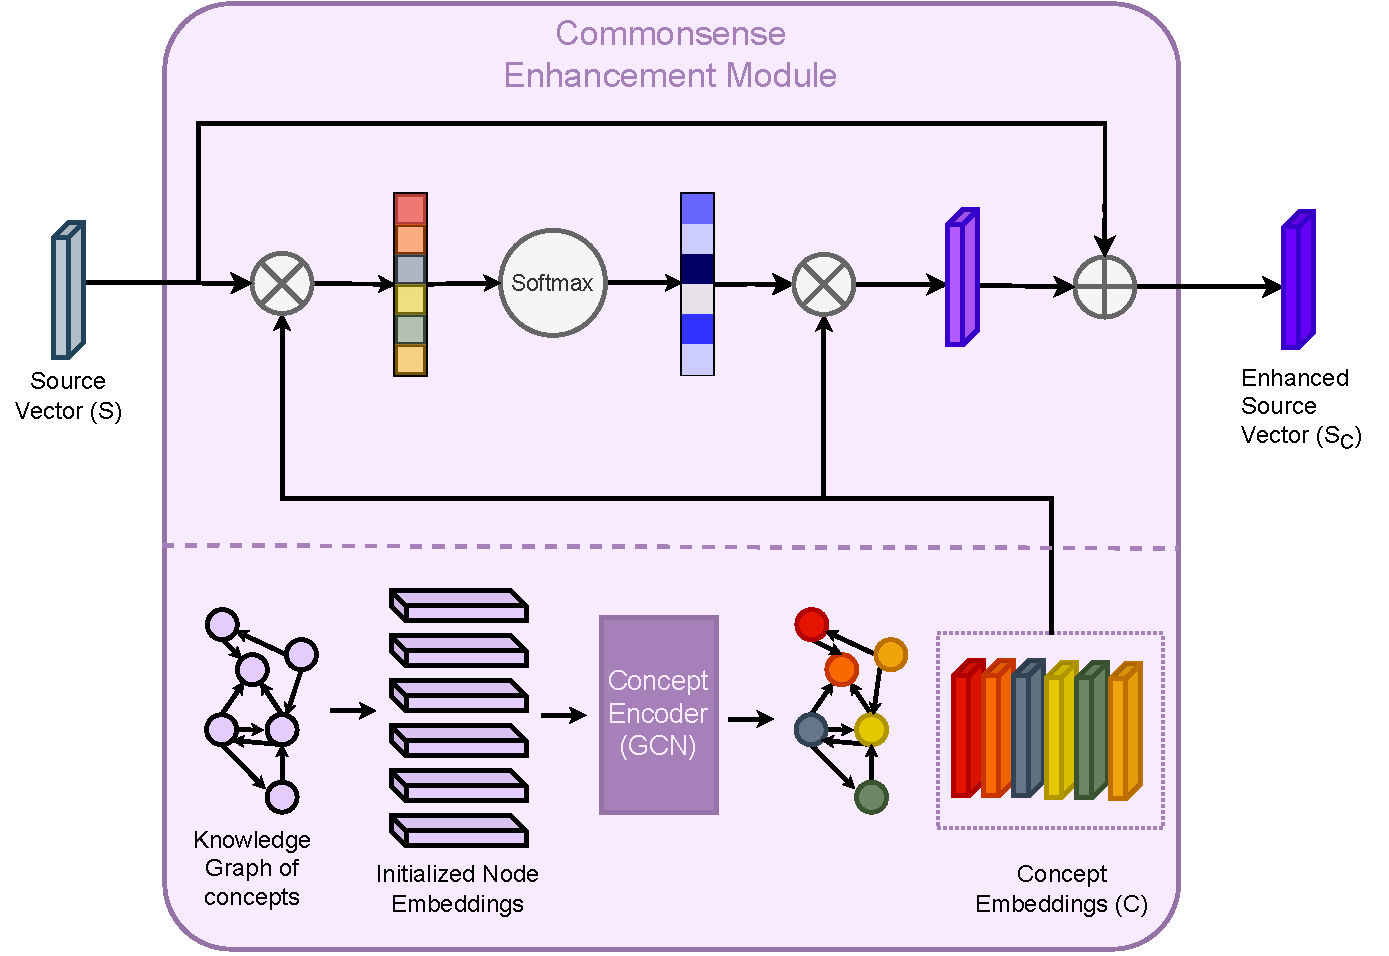
\includegraphics[width=0.8\linewidth]{figures/figure_files/Cem.pdf}
    \caption{\modelname Commonsense Enhancement Module (CEM). CEM comprises a concept encoder and an enhancement mechanism that uses the previously encoded concept vectors to update a given input vector (video/query vectors). The concept encoder employs a Graph Convolution Network for encoding the nodes (concepts) of \(G_C\). 
    }
  \label{fig:cem}
\end{figure}

CEM includes a set \(C\!=\!\left\{c_{1}, c_{2}, \dots, c_{n_{C}}\right\}\) of \(n_{C}\) concept vectors, where \(c_{i} \in \mathbb{R}^{d}\) and \(d\) is the concept feature dimension (same dimension as $\forall v_i \in V$ and $\forall q_i \in Q$). In general, given source feature vectors $S\!=\!\left\{ s_{1},s_{2},\ldots,s_{n}\right\}$ with individual feature vectors $s_{i \in [1,n]} \in \mathbb{R}^{d}$, the enhanced feature vectors $S_{C}$ are obtained using a commonsense enhancement mechanism $\phi_{C}$.
We implement this commonsense enhancement step $\phi_{C}$ as a cross-attention mechanism that enriches source input features, attending over $S$ guided by the commonsense concept vectors $C$, \ie, 
\begin{equation}
\label{eq:cenhance}
\scalemath{1}{
    }
    S_{C} = S + \phi_{C}(S) = S + \sigma \left( \frac{SW_{Q}(CW_{K})^{T}}{\sqrt{d}} \right) C W_{V},
\end{equation}
where $\sigma$ is a softmax activation, \(W_{Q}\), \(W_{K}\), \(W_{V}\) are trainable matrices and \(d\) is the common dimension of the vectors \(S\) and \(C\). In our setting, the source feature vectors $S$ are either video $V$ or pseudo-query $Q$ features. We build separate enhancement mechanisms for $V$ and $Q$, \ie, the projection matrices \(W_{Q}\), \(W_{K}\), \(W_{V}\) are not shared between $Q$ and $V$. We elaborate more on the rationale in the appendix.
The enriched video and pseudo-query features are denoted as \(V_{C}\!=\!\phi_{C_{\text{vid}}}(V)\) and \(Q_{C}\!=\!\phi_{C_{\text{pq}}}(Q)\), respectively.

\paragraph{Concept Encoder.}
The concept vectors \(C\) mentioned above are feature representations that internally form the nodes of the commonsense graph, \(G_C\). Accordingly, graph \(G_{C}\) is represented as a matrix, where \(G_{C(i,j)}\) represents the total number of directed relational edges between \(c_{i},c{j} \in C\) that start at \(c_i\) and end at \(c_j\). To encode the commonsense information, we employ Graph Convolutional Networks (GCN) \cite{hammond_wavelets_2011}. The concept encoder is composed of $L$ graph convolution layers, each of which performs a convolution step
\begin{equation}
\scalemath{1}{
    C^{\left(l+1\right)}=\sigma \left( AC^{\left(l\right) }W^{\left( l\right) }\right),
    }
\end{equation}
where $C^{\left(l\right)}$ are node (concept) features and $W^{\left( l\right)}$ trainable weight matrix of layer $l \in [1, L]$, $\sigma$ is a nonlinear activation function, and $A$ is the adjacency matrix obtained by normalizing graph $G_C$ with the degree matrix $D$. Since $G_C$ is a directed graph, normalization can be formulated as $A\!=\!D^{-1}G_{C}$.

\paragraph{Commonsense Information.}
We use ConceptNet \cite{speer_conceptnet_2017}, a popular knowledge graph that provides information spanning various types of relationships such as physical, spatial, behavioral, \etc To ensure that the ConceptNet information utilized is relevant to themes found in the video data, we consider the set of objects available in pseudo-queries and include the top-$k$ most frequently occurring objects to be the seed concept set \(C\). We extract the  ConceptNet subgraph that includes all edges incident between the concepts in \(C\). 
We filter the edge types based on a pre-determined relation set \(R\), which is compiled to involve relations that are relevant to the nature of the video localization task, \eg, spatial (\textit{AtLocation}, \etc) and temporal (\textit{HasSubevent}, \etc) relations are useful for video understanding, while \textit{RelatedTo} and \textit{Synonym} are fairly generic relations that add little information to the localization task. Table \ref{tab:relations} shows the relations included in \(G_C\).

\paragraph{Cross-Modal Interaction Module.} The commonsense enriched video and query features, \(V_{C}\) and \(Q_{C}\), are fused with a multi-modal cross-attention mechanism. We employ a two-step fusion process. First, Query-guided Video Attention (QVA) is applied to attend over video $V_C$, and Video-guided Query Attention (VQA) attends over query $Q_C$ guided by video $V_C$, resulting in updated features $V_C'$ and $Q_C'$, respectively. Both QVA and VQA utilize Attention Dynamic Filters~\cite{rodriguez_proposal-free_2020} that adaptively modify video features, dynamically adjusting them in response to the query, and vice versa. Next, the attended features are fused using a cross-attention mechanism over $V_C'$ guided by $Q_C'$, resulting in localized video features $V_{C_{\text{loc}}}$.

\paragraph{Temporal Regression Module.}
The final step involves a regression layer that approximates $\hat{V}_{\text{span}}$. We employ attention-guided temporal regression to estimate the span of the target video moment. To find important temporal segments relevant to the query, the fused features $V_{C_{\text{loc}}}$ are temporally attended based on the query features to obtain $V_{\text{ta}}$. Then, the span boundaries are localized using a regressor implemented as a Multi-Layer Perceptron (MLP).

\begin{align}
{o}_i = \sigma\left({W}_{1} V_{C_{\text{loc}_i}} + {b}_{{1}}\right) \\
V_{\text{ta}} = \sum_{i=1}^{T} o_i V_{C_{\text{loc}_{i}}} \\
[\hat{t}_s, \hat{t}_e] = {W}_2 {V}_{\text{ta}} + {b}_{2}.
\end{align}
Here, ${W}_{1}$ and ${b}_1$ are the weight matrix and bias vector of the temporal attention MLP, $\sigma$ represents the sigmoid activation function, $V_{C_{\text{loc}_i}}$ stands for the encoded localized video features, ${V}_{\text{ta}}$ represents the temporally attended video features, ${W}_2$ and ${b}_2$ denote the weight matrix and bias vector of the regression MLP, and $[\hat{t}_s, \hat{t}_e]$ correspond to the start and end timestamps of the predicted video span $\hat{V}_{\text{span}}$.

\begin{table}[t!]
\centering
\resizebox{\linewidth}{!}{
\begin{tabular}{ll}
\toprule
\textbf{Category} & \textbf{Relations}                                                                                         \\ \toprule
Spatial           & AtLocation, LocatedNear                                                                                    \\ \midrule
Temporal          & \begin{tabular}[c]{@{}l@{}}HasSubevent, HasFirstSubevent, HasLastSubevent, HasPrerequisite\end{tabular} \\ \midrule
Functional        & UsedFor                                                                                                    \\ \midrule
Causal            & Causes                                                                                                     \\ \midrule
Motivation        & MotivatedByGoal,  ObstructedBy                                                                             \\ \midrule
Other             & CreatedBy, MadeOf                                                                                          \\ \midrule
Physical          & \begin{tabular}[c]{@{}l@{}}HasA, HasProperty, Antonym, SimilarTo\end{tabular}                      
\\ \bottomrule
\end{tabular}
}

\caption{Relations in the Commonsense Enhancement Module (CEM) grouped by categories.}
\label{tab:relations}

\end{table}
\subsection{Training and Inference}
The training objective is 
$\mathcal{L}_{loc} = \mathcal{L}_{treg}+\lambda \mathcal{L}_{ta},$ where \(\lambda\) is a balancing hyperparameter, \(\mathcal{L}_{ta}\) is a temporal attention guided loss and \(\mathcal{L}_{treg}\) is the regression loss.  The temporal attention-guided loss is defined as
\begin{equation}
\label{tatt}
\mathcal{L}_{ta} = \frac{\sum^{T}_{i=1}g_{i}\log \left( a_{i}\right)}{\sum^{T}_{i=1}g_{i}},
\end{equation}
where \(a_{i}\) is the attention weight for video frame \(v_{i}\) and \(g_{i}\) is the attention mask for \(v_{i}\), that is assigned to \(1\) if \(v_{i}\) is inside the target video segment, and \(0\) otherwise. 
This objective encourages the model to produce higher attention weights for video segments that are relevant to the query. 
On the other hand, \(\mathcal{L}_{treg}\) dictates the video span boundary regression and is the sum of smooth $\ell_1$ distances between start and end timestamps of the ground truth and predicted spans, \ie,
\begin{equation}
\label{treg}
\mathcal{L}_{treg} = \text{smooth}{\ell_1}(t_{s}, \hat{t}_{s}) + \text{smooth}{\ell_1}(t_{e}, \hat{t}_{e}).
\end{equation}
Here, $t_{s}$ and ${t}_{e}$ represent the ground truth start and end timestamps and $\hat{t}_{s}$ and $\hat{t}_{e}$ the predicted start and end timestamps, respectively.
The integration of a smoothing mechanism enhances training stability and improves the model's ability to handle outliers. Finally, during inference, we employ an off-the-shelf part-of-speech tagger to extract nouns from the text input query and feed them as query input to the trained \modelname video localizer.